\noindent\textbf{Directions}: You are advised to spend the first 5 minutes
reading all of the questions and planning your answers. You will then
have 10 minutes to answer all three of the following questions. You may
begin writing your responses before the reading period is over. It is
suggested that you spend approximately half your time on the first
question and divide the remaining time equally between the next two
questions. Include correctly labeled diagrams, if useful or required, in
explaining your answers. A correctly labeled diagram must have all axes
and curves clearly labeled and must show directional changes. If the
question prompts you to “Calculate,” you must show how you arrived at
your final answer. Use a pen with black or dark blue ink. \\

\clearpage
\begin{enumerate}[itemsep=0.5cm]
      \item
            \begin{figure}[h]
                  \centering
                  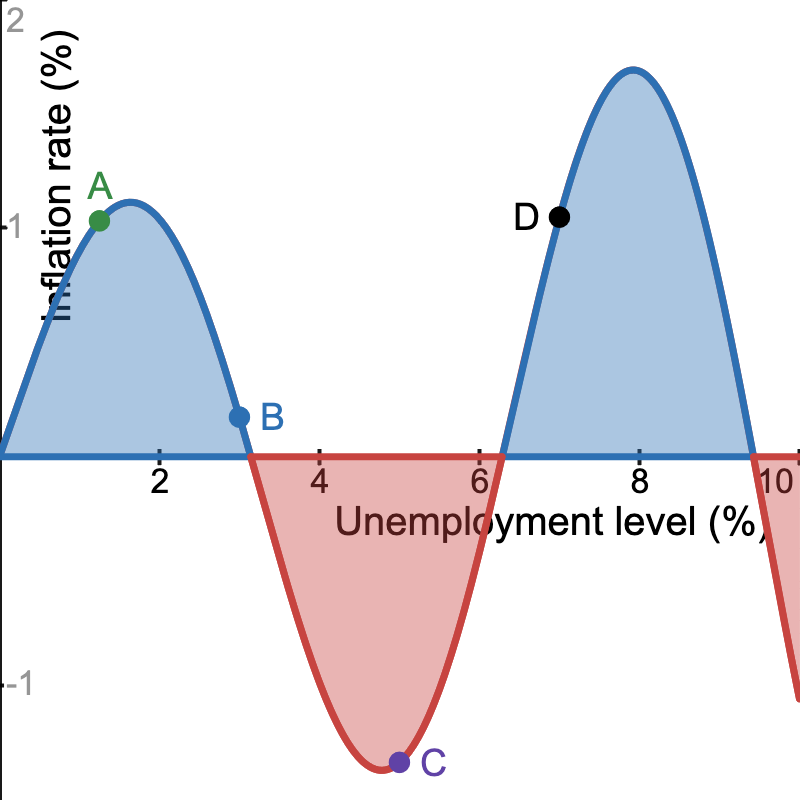
\includegraphics[width=0.4\textwidth]{assets/phillips.png}
            \end{figure}

            \[
                  f\left(x\right)=\sin\left(x\right)e^{x/15}
            \]

            At a campaign event, Barack Obama was confronted with a voter
            named Joe who was unemployed and complaining about rampant
            inflation during the Obama regime. Joe claimed that he was
            paying too much tax and became a martyr among conservative
            circles, known as ``Joe the Plumber'' (RIP). \\
            \medskip

            Consider the above graph, which represents the Phillips Curve
            during Obama's 2-term presidency. Answer the following questions:\@

            \bigskip

            \begin{adjustwidth}{0.3in}{0.3in}
                  \begin{enumerate}[itemsep=0.5cm]

                        % integral represents misery index
                        % point b maximizes misery index
                        \item Identify the point on the Philips curve that best
                              corresponds to Obama's fiscal policy, assuming that
                              what Joe is saying is correct and assuming that Joe
                              represents the average American.
                        \item Identify the central relationship between inflation
                              and unemployment that is the basis for the Philips Curve.

                        \item Given what we know about Joe, extrapolate this
                              information to determine whether the overall unemployment
                              rate during the Obama regime is high or low by traditional
                              American standards.

                              \clearpage

                        \item
                              In the 1970s, Arthur Okun, economic adviser to
                              President Lyndon B. Johnson, proposed the ``Misery
                              Index'' as an indicator of economic
                              health~\cite{inflationdata}. It's defined as
                              $Unemployment\,Rate \times Inflation\,Rate$

                              \begin{enumerate}
                                    \item If we were to evaluate $\displaystyle \int f(x) \,
                                                \differential x$, what would it represent?

                                    \item Develop a strategy for evaluating the misery
                                          index at a point using the Taylor Series
                                          approximation of $f(x)$. What Maclaurin series do
                                          you need to manipulate to develop a Taylor series
                                          approximation for $f(x)$?

                                    \item Use the Taylor remainder theorem to determine
                                          how many terms you need to add or multiply in order
                                          to ensure that your estimation of the misery index
                                          is accurate to within two decimal places.

                                    \item Identify the point ($A$, $B$, $C$, or
                                          $D$) on the graph which maximizes the misery
                                          index.
                              \end{enumerate}
                        \item Assume that Joe's complaints are valid. Determine null
                              and alternate hypotheses relating to the inflation rate
                              given what we know about Joe's situation.

                        \item Given a random sample of $n$ Americans, $p$ percentage
                              of them agree with Joe's assumptions. At what value of
                              $p$ can we conclude that there is a statistically
                              significant reason to reject the null hypothesis $H_0$
                              (at the $\alpha = 0.05$ confidence level)?

                        \item Interpret your conclusions from parts (f) and (d) and
                              state the result. With what confidence and accuracy can we
                              assess the misery index?

                        \item Identify the potential consequences of a Type I error
                              in this scenario and what can be done, if anything, to
                              resolve it. What about a Type II error?
                  \end{enumerate}
            \end{adjustwidth}
\end{enumerate}